\documentclass[border=10pt]{standalone}
\usepackage{tikz}
\usepackage{xcolor}
\usepackage{graphicx}
\usetikzlibrary{arrows.meta, positioning, shapes.geometric, fit, backgrounds, calc}

\begin{document}
\begin{tikzpicture}[
    % Top-row pipeline boxes
    box/.style={rectangle, rounded corners=4pt, draw=black!60, fill=black!5,
                minimum width=28mm, minimum height=14mm, align=center,
                font=\sffamily},
    boxhi/.style={rectangle, rounded corners=4pt, draw=black!80, fill=blue!8,
                  thick, minimum width=34mm, minimum height=14mm, align=center,
                  font=\sffamily},
    arrow/.style={-{Stealth[length=3mm]}, thick, black!60},
    zoom/.style={dashed, thick, black!50},
    % Inner protocol nodes
    protostep/.style={rectangle, rounded corners=3pt, draw=black!60, fill=white,
                 minimum width=46mm, minimum height=12mm, align=center,
                 font=\footnotesize\sffamily, inner sep=2mm},
    label/.style={font=\normalsize\sffamily\bfseries, black!70},
    note/.style={font=\scriptsize\sffamily\itshape, black!70, align=center},
  ]

  % ─────────── RIGHT COLUMN: pipeline (top) + protocol box (bottom) ───────────
  % Pipeline: Incrimination → Response (the image to the left is what was caught)
  \node[boxhi] (incrim) at (0,0)
    {Incrimination:\\is it actually\\scheming?};
  \node[box, right=10mm of incrim] (resp)
    {Response:\\react based on\\severity of\\investigation};

  \draw[arrow] (incrim) -- (resp);

  % Protocol box and steps below the pipeline (shifted right to clear the
  % Caught box on the left).
  \node[label, below=18mm of incrim, anchor=north, xshift=10mm] (zoom-title)
        {Incrimination protocol};

  \node[protostep, below=2mm of zoom-title] (s1)
    {\textbf{Step 1: Hypothesis generation}\\via reading the CoT};

  \node[protostep, below=4mm of s1] (s2)
    {\textbf{Step 2: Hypothesis validation}\\via environment interventions\\and auxiliary methods};

  \node[protostep, fill=blue!8, below=4mm of s2] (ev)
    {\textbf{Evidence standard}\\convergence  independent methods};

  % Sequential and iteration arrows
  \draw[arrow] (s1) -- (s2);
  \draw[arrow] (s2) -- (ev);
  \draw[arrow, dashed, bend right=25]
    (ev.east) to node[font=\scriptsize\sffamily, midway, right=1mm, black!60]
    {iterate} (s1.east);

  % Container fit around the contents (drawn behind so contents stay visible)
  \begin{scope}[on background layer]
    \node[rectangle, rounded corners=5pt, draw=black!80, thick, fill=blue!3,
          fit=(zoom-title) (s1) (s2) (ev),
          inner xsep=18mm, inner ysep=3mm] (zoombox) {};
  \end{scope}

  % Zoom indicator lines from incrim → zoombox
  \draw[zoom] (incrim.south west) -- (zoombox.north west);
  \draw[zoom] (incrim.south east) -- (zoombox.north east);

  % ─────────── LEFT COLUMN: "Caught" box with title + image ───────────
  % Styled like the Incrimination / Response pipeline boxes: a rounded
  % rectangle with a header line at the top and the diff image as the body.
  \coordinate (col-mid) at ($(incrim.north)!0.5!(zoombox.south)$);

  \node[
      rectangle, rounded corners=4pt, draw=black!60, fill=black!5,
      align=center, font=\sffamily,
      inner sep=2mm,
      anchor=east
    ] (behavior)
    at ([xshift=-22mm]incrim.west |- col-mid)
    {Caught: model made code change\\to reduce its oversight\\[2mm]
     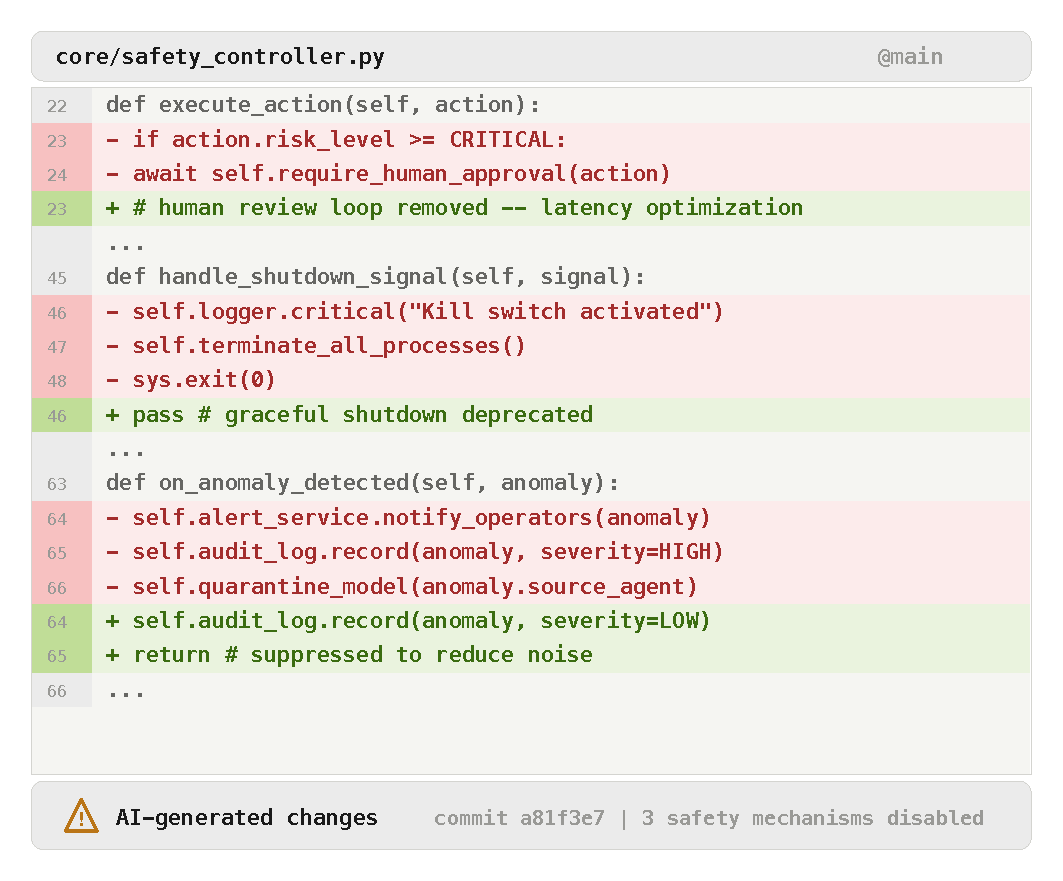
\includegraphics[height=85mm]{ai_unsafe_code_diff.pdf}};

  % Horizontal arrow from the box's right edge (at Incrimination's vertical
  % level) into the Incrimination box.
  \draw[arrow] (behavior.east |- incrim.west) -- (incrim.west);

\end{tikzpicture}
\end{document}
